% adapted from:
% NOAOPROP.TEX -- template for NOAO STANDARD telescope proposals.
% Revised for the 2018A semester (February - July 2018)
% For later semesters, the current form may be obtained from our Web
% page at http://www.noao.edu/noaoprop/noaoprop.html

% Please do not modify or delete this line.
\documentclass[11pt]{article}
\usepackage{nprop30}
\usepackage{graphicx}
\usepackage{natbib}
\bibliographystyle{abbrvnat}

% Please do not modify or delete this line.
\begin{document}

% Uncomment the following line and enter a previous semester and ID
% (e.g. 01B-0987) if you wish to flag this proposal as a resubmission
\pastid{}

% Please do not modify or delete this line.
\proposaltype{}

%%%%%%%%%%%%%%%%%%%%%%%%%%%%%%%%%%%%%%%%%%%%%%%%%%%%%%%%%%%%%%%%%%%%%

% SCIENTIFIC CATEGORIES
%
% Please select a "scientific category" that best describes your
% program by uncommenting only ONE of the selections below.  Your
% \sciencecategory selection will be used to assign a review panel to
% your proposal.  DO NOT MODIFY THE SELECTION YOU UNCOMMENT.  A
% description of each of these categories is available on our Web page
% at https://www.noao.edu/noaoprop/help/scicat.html

% EXTRA-GALACTIC LIST (do not uncomment this line)
%\sciencecategory{Active Galaxies}
%\sciencecategory{Cosmology}
%\sciencecategory{Large Scale Struc.}
%\sciencecategory{Clusters of Galaxies}
%\sciencecategory{High Z Galaxies}
%\sciencecategory{Low Z Galaxies}
%\sciencecategory{Resolved Galaxies}
%\sciencecategory{Stellar Pops (EGAL)}
%\sciencecategory{EGAL - Other}

% GALACTIC/LOCAL GROUP LIST (do not uncomment this line)
\sciencecategory{Star Clusters}
%\sciencecategory{Stellar Pops (GAL)}
%\sciencecategory{HII Reg., PN, etc.}
%\sciencecategory{ISM}
%\sciencecategory{Star Forming Regions}
%\sciencecategory{Young Stellar Obj.}
%\sciencecategory{Massive Stars}
%\sciencecategory{Low Mass Stars}
%\sciencecategory{Stellar Remnants}
%\sciencecategory{Galactic - Other}

% SOLAR SYSTEM LIST (do not uncomment this line)
%\sciencecategory{Kuiper Belt Objects}
%\sciencecategory{Small Bodies \& Moons}
%\sciencecategory{Planets}
%\sciencecategory{Extrasolar Planets}
%\sciencecategory{Solar System - Other}

% KEYWORDS (1-5 keywords are required for Gemini).  Note that the keywords
% are different for the extra-galactic, galactic and solar system lists
% above, so if you change your science catagory you will need to check to
% be certain your keywords are still valid (see the list of keywords at
% http://www.noao.edu/noaoprop/help/keywords.html).
%\geminidata{keyword1}{Galactic halo}
%\geminidata{keyword2}{Globular clusters}

%%%%%%%%%%%%%%%%%%%%%%%%%%%%%%%%%%%%%%%%%%%%%%%%%%%%%%%%%%%%%%%%%%%%%%

% TITLE
%
% Give a descriptive title for the proposal in the \title command.
%
% Note that a title can be quite long; LaTeX will break the title into
% separate lines automatically.  If you wish to indicate line breaks
% yourself, do so with a `\\' command at the appropriate point in
% the title text.  Use both upper and lower case letters (NOT ALL CAPS).

\title{Catchy Title}


%%%%%%%%%%%%%%%%%%%%%%%%%%%%%%%%%%%%%%%%%%%%%%%%%%%%%%%%%%%%%%%%%%%%%%

% ABSTRACT
%
% Give a general abstract of the scientific justification appropriate
% for a non-specialist.  Write between the \begin{abstract} and 
% \end{abstract} lines.  Limit yourself to approximately 175 words.
% Abstracts of accepted proposals will be made publicly available.

% DO NOT remove the \begin{abstract} and \end{abstract} lines.

\begin{abstract}
%This sample proposal offers tips on how to prepare your telescope
%proposal for observing on facilities available through NOAO. 
%With the NOAO Proposal Form, you can apply for time on the 
%Gemini North and South Telescopes, the  Hobby-Eberly
%Telescope, the 6.5-m telescope of the MMT Observatory, and the telescopes
%at the Cerro Tololo Inter-American Observatory and the Kitt Peak
%National Observatory.  

Your abstract is the review panel's window into your proposal: the abstract
provides an initial impression about your proposal and it is also
what panel members refer to at the review meeting to remind themselves
about the content of your proposal.  Take advantage of the opportunity
to give the panel members an understandable and concise summary of what 
you want to do, and why.  Write your abstract so that non-specialists can
quickly understand why the observations you want to make are important.

\end{abstract}

%%%%%%%%%%%%%%%%%%%%%%%%%%%%%%%%%%%%%%%%%%%%%%%%%%%%%%%%%%%%%%%%%%%%%%

%%%
%%% For the archival proposal, fill out only the following:
%%% - Telescope / Instrument you request 
%%%

% SUMMARY OF OBSERVING RUNS REQUESTED
%
% List a summary of the details of the observing runs being requested,
% for UP TO SIX runs.  The parameters for each run are segregated
% between \begin{obsrun} and \end{obsrun} lines.  Please be sure
% that the information is isolated properly for each run.
%
%   \begin{obsrun}
%   \telescope{}        % For example, \telescope{KP-4m}
%   \instrument{}       % For example, \instrument{ECHUV + T2KB}
%   \numnights{}        % For example, \numnights{6}
%   \lunardays{}        % For example, \lunardays{grey}
%   \optimaldates{}     % For example, \optimaldates{Sep - Nov}
%   \acceptabledates{}  % For example, \acceptabledates{Aug - Jan}
%   \end{obsrun}
%
% The following telescope identifiers MUST be used in the \telescope{}
% field.  Some of the telescope identifiers must include an observatory
% code as well.
%
% CTIO: CT-4m, SOAR, CT-1.3m, CT-0.9m
% KPNO: WIYN, KP-0.9m
% AAO: AAT
% LCO: LCO-2m, LCO-1m
% CHARA: CHARA
%
% Select the instrument and detector identifiers from the list on our
% Web page at https://www.noao.edu/noaoprop/help/facilities.html.
% The correct codes MUST be used to ensure your correct
% instrument + detector combination.
%
% \numnights should give the number of nights of the run (for queue
% observations, use fractional 10-hour equivalent nights, e.g.
% 3 hours = 0.3 nights).  Formats such as 5x0.5 are acceptable.
%
% \lunardays should contain the word "darkest", "dark", "grey", or
% "bright", which in turn reflects the number of nights from new moon
% where darkest<=3, dark<=7, grey<=10, bright<=14.  Particular lunar 
% phase requirements dictated by the science program (e.g., "<=12", 
% "+9, -6", or "full moon more than 2 hours away from Taurus") should
% be noted in the "scheduling constraints or non-usable dates" section 
% below.
%
% \optimaldates should contain the range of OPTIMAL months, as shown 
% below.
%
% \acceptabledates should give the range of ACCEPTABLE months (i.e.,
% you would not accept time outside those limits).
% NOTE THAT DUE TO INSTRUMENT BLOCKING RESTRICTIONS YOU SHOULD MAKE 
% THIS RANGE AS GENEROUS AS POSSIBLE.
%
% For QUEUE-SCHEDULED observations, you may set the date range to the 
% full semester range and set \lunardays to the brightest moon your
% observations could tolerate if the program were scheduled classically.
%
% To enter the acceptable and optimal date ranges, please use two
% dash-separated months with 3-letter abbreviations for the month
% (Jan, Feb, Mar, Apr, May, Jun, Jul, Aug, Sep, Oct, Nov, Dec).
% For example:  \optimaldates{Nov - Dec}.
% We appreciate your help in not using vague range specifications
% like "October dark run" or "mid-January" which will require human
% intervention.
%
% FOR LONGTERM STATUS PROPOSALS SPECIFY ONLY THE RUNS FOR THE CURRENT
% SEMESTER, AND NOT FOR ANY SUBSEQUENT SEMESTERS.

% DO NOT remove any of the \begin{obsrun} and \end{obsrun} blocks, 
% even if the blocks are empty.

\begin{obsrun}
\telescope{14-inch}
\instrument{STL-1001E}
\numnights{1}
\lunardays{dark}
\optimaldates{Oct. 27}
\acceptabledates{Oct. 27, Nov. 7}
\end{obsrun}

\begin{obsrun}
\telescope{14-inch}
\instrument{STL-1001E}
\numnights{0.5}
\lunardays{grey}
\optimaldates{Oct-Nov}
\acceptabledates{Oct-Nov}
\end{obsrun}

\begin{obsrun}
\telescope{}
\instrument{}
\numnights{}
\lunardays{}
\optimaldates{}
\acceptabledates{}
\end{obsrun}

\begin{obsrun}
\telescope{}
\instrument{}
\numnights{}
\lunardays{}
\optimaldates{}
\acceptabledates{}
\end{obsrun}

\begin{obsrun}
\telescope{}
\instrument{}
\numnights{}
\lunardays{}
\optimaldates{}
\acceptabledates{}
\end{obsrun}

\begin{obsrun}
\telescope{}
\instrument{}
\numnights{}
\lunardays{}
\optimaldates{}
\acceptabledates{}
\end{obsrun}


% If there are scheduling constraints or non-usable dates for any of
% the runs specified, (i.e., other than the default lunar phase 
% requirements or when your object is up) please give the dates by 
% filling in the curly braces in \unusabledates{}.  Note here if you 
% are requesting runs in an "either/or" situation, e.g. run 1 or run 2, 
% but not both. This is also the place to advise us of any special 
% constraints which affect the scheduling of your observing run (e.g. 
% "schedule run #1 before run #2" or "run dates must be coordinated 
% with HST observations").
% 
% Please limit your text to six lines on the printed copy.

\unusabledates{Run 1 needs to be scheduled to catch phase 0 of the eclipsing binary.  Run 2: please avoid Oct. 25 (proposers have a mid-term the next morning).}

%%%%%%%%%%%%%%%%%%%%%%%%%%%%%%%%%%%%%%%%%%%%%%%%%%%%%%%%%%%%%%%%%%%%%%%

%%%
%%% Blind review - do not list your name
%%%

% INVESTIGATOR'S (PI AND CoI) INFORMATION BLOCKS
%
% Please give the PI's name (first name first followed by middle
% initial and last name), affiliation, department and complete mailing
% address, as well as an email address.  Also give a complete phone
% number, and a number for a fax machine if you have access to one.
% You must also indicate the principal investigator's status with one
% of the one-letter codes inside the \invstatus{} curly braces, as
% indicated below.
%
% The affil{}, \department{}, \address{} (use a comma separate list as
% needed), \city{}, \state{}, \zipcode{}, and \country{} (for non-US
% addresses) fields will be used together as your full postal mailing
% address.  Please be sure this information is complete.  Note that
% some institutions will not deliver postal mail if a department is
% not included in the postal mailing address.  Non-US addresses should
% include the country and any local postal codes.
%
% The fax number does not print on the form.
%
% For each CoI please include a name, affiliation, email address and
% investigator's status within the \begin{CoI} and \end{CoI} lines.
%
% For each \invstatus{} field, please fill in the appropriate
% investigator status code from the following list.  If the investigator
% is a graduate student, indicate "T" if THIS proposal is related to a
% thesis project, or "G" otherwise.  This code should represent the
% status of the individuals at the time of the proposal submission.
% This information is necessary to assist us with our required reporting
% to the NSF.
%
% \invstatus{P} % investigator has obtained PhD or equivalent
% \invstatus{T} % investigator is grad student, proposal is thesis
% \invstatus{G} % investigator is grad student, proposal not thesis
% \invstatus{U} % investigator is an undergraduate student
% \invstatus{O} % investigator has other status (none of the above)
%
% DO NOT remove the \begin{PI} and \end{PI}.  Only one individual's
% name per \name field is allowed.
%
% Investigator names will now appear on page 2 of the printed proposal.
% Do not remove this line.
%\investigators
%
%\begin{PI}
%\name{George W. Bush}
%\affil{Office of the President}
%\department{}
%\address{1600 Pennsylvania Avenue}
%\city{Washington}
%\state{DC}
%\zipcode{20500}
%\country{}
%\email{president@whitehouse.gov}
%\phone{(202) 456-1414}
%\fax{(202) 456-2883}
%\invstatus{O}
%\end{PI}
%
%\begin{CoI}
%\name{Condoleeza Rice}
%\affil{Dept. of State}
%\email{secretary@state.gov}
%\invstatus{P}
%\end{CoI}
%
%\begin{CoI}
%\name{Nancy Pelosi}
%\affil{U.S. House of Representatives}
%\email{sf.nancy@mail.house.gov}
%\invstatus{O}
%\end{CoI}

%\begin{CoI}
%\name{}
%\affil{}
%\email{}
%\invstatus{}
%\end{CoI}

%\begin{CoI}
%\name{}
%\affil{}
%\email{}
%\invstatus{}
%\end{CoI}


%%%%%%%%%%%%%%%%%%%%%%%%%%%%%%%%%%%%%%%%%%%%%%%%%%%%%%%%%%%%%%%%%%%%%%

% In the following "essay question" sections, the delimiting pieces of
% markup (\justification, \expdesign, etc.) act as LaTeX \section*{}
% commands.  If the author wanted to have numbered subsections within
% any of these, LaTeX's \subsection could be used.
%
% DO NOT REDUCE THE FONT SIZE, and do not otherwise fiddle with the
% format to get more on a page.  We will reset any changes back to the
% default font.

% SCIENTIFIC JUSTIFICATION
%
% Give the scientific justification for the proposed observations.
% This section should consist of paragraphs of text followed by any
% references and up to three figures and captions.  Be sure to include
% overall significance to astronomy.  THE SCIENTIFIC JUSTIFICATION
% SHOULD BE LIMITED TO ONE PAGE (the review panels have requested that
% we not send them more than one page), with up to two additional pages
% for references, figures (no more than three), and captions. 

% You can include references through BibTeX.

\sciencejustification
The scientific justification should explain the overall goals of
your program in the context of your field, as well as the importance
of your program to astronomy.
Writing a good scientific justification is an art.  It takes
skill and practice.  And it requires a good scientific idea.
This last you must supply but a few general guidelines
about proposal writing might still be helpful...

\begin{itemize}
\item
State succinctly and clearly the problem you are trying to solve
and the progress that will be made toward doing so if the proposed
observations are successful.  If the review panel members have to work hard
even to understand what you want to do, they are unlikely to be
sympathetic to your proposal.

\item
Explain clearly why the project is important and how it
relates to the broad context and important issues in your field.
Many proposals focus too tightly on a specific observational
goal (e.g. ``measure the velocity dispersion of this cluster of galaxies'')
without explaining why it is important or how it relates to a
significant question about the Universe.

\item
Be specific.  If your observations will ``constrain theoretical
models,'' then discuss what will be constrained and why those
constraints matter.  Make sure the review panel understands exactly why
the observations you propose will make a difference in your field,
and exactly how the observations will refine or
require changes in the theory.

\item
Keep it simple.  Try to focus on the central idea of your proposal.
Complex arguments are hard to explain and hard for the panel members to follow.
Distracting tangential arguments obscure the theme of your proposal.

\item
Include a figure to help explain what you want to do.  Sample
data or model predictions shown in a figure often help clarify
complex arguments for the panel members.  A sample figure is included
below with this proposal.

\item
Keep it short.  Never exceed a page for the text of the scientific
justification, and never reduce the font size.  It may even help to
be a little under a page, and increase the font size a little!
Organize your presentation with paragraphs, headings, and bullets
so it is easy to read.

\item
Include and check references as appropriate \citep{Bell96}.

\item
Print out the proposal to be sure your LaTeX is correct.
Proofread it.  Make sure the proposal is correct scientifically,
technically, and grammatically.  Run a spellchecker.

\end{itemize}

Finally, when an opportunity arises, volunteer to serve on
a TAC or review panel.  The experience is a great help in
learning how to write a good scientific justification.

\bibliography{proposal_refs}

\begin{figure}[hbt]
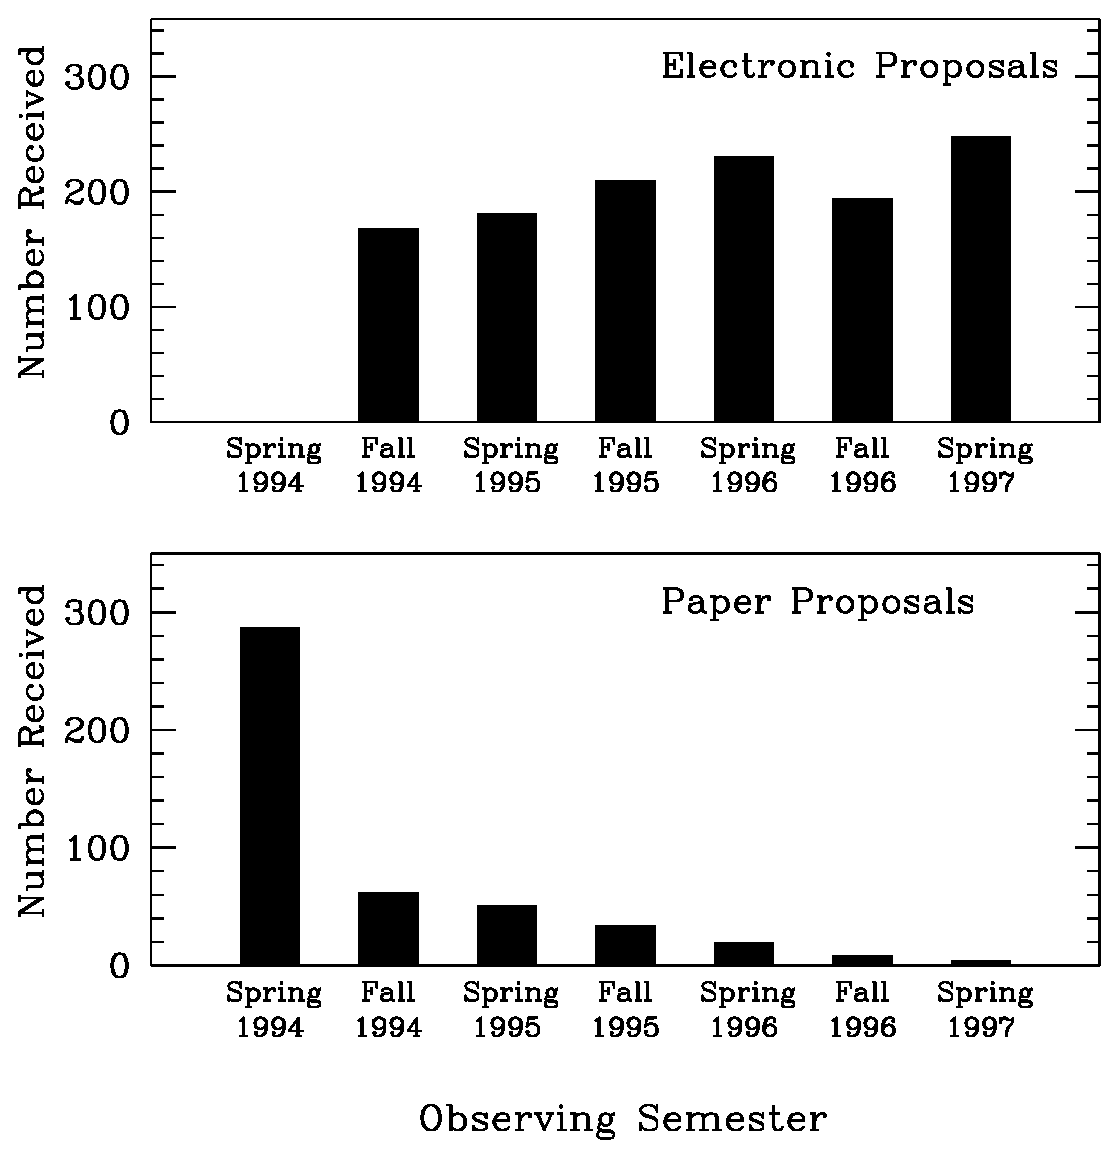
\includegraphics[width=0.5\hsize]{figure1a.eps}
\caption{This sample figure shows how quickly electronic proposals
for telescope time replaced paper ones.}
\end{figure}


\clearpage


% TECHNICAL JUSTIFICATION
% (EXPERIMENTAL DESIGN)
%
% This section should consist of text only (no figures).
% There is a limit of one page of printed text.

% Describe your overall observational program.  How will these 
% observations contribute toward the accomplishment of the goals 
% outlined in the science justification?  If you've requested 
% long-term status, justify why this is necessary for successful 
% completion of the science.
%
% NOTE: In previous versions of the proposal form, this section
% requested details about the use of non-NOAO observing facilities. 
% Such information should now be entered in the following "Other
% Facilities" section.

\expdesign
The review panel looks to this section to find out about the overall
strategy of your data analysis.  You need to convince the panel that your strategy will be successful.  If the strategy is found to be infeasible, the proposal will be outright rejected.

\begin{itemize}
  
\item
  What are the target objects and target datasets, and how were they selected?

\item
  Comment on the observability of your targets.

\item
  Provide a detailed explanation of the exposure time estimate.  Also provide an estimate of how long your total observing session will take (with multiple exposures, calibration, etc.).

\item
  Provide an explanation of which filter(s) you will use.
  
\item
  What calibration data will you require?

\item
  Will you require external data?  If so, describe the nature of that dataset, and how you will analyze it.
  
\item
  What do you plan to measure, and how?

\end{itemize}
 


% PROPRIETARY PERIOD
% 
% Enter the proprietary period for your data between the braces.
% The normal duration is 18 months from when the data are taken at
% the telescope.  Requests for longer proprietary periods must
% be approved by the NOAO Director.

%\proprietaryperiod{18 months}


% OTHER FACILITIES OR RESOURCES
% 
% This section should consist of text only (no figures).
% Please limit to about a half page of printed text.
% 
% 1) We are interested in understanding how observations made through
% NOAO observing opportunities complement or support data from other
% facilities both on the ground and in space.   We will use this
% information to guide the evolution of the NOAO program; it will not
% affect the success of your proposal in the evaluation process.
% Please describe how the proposed observations complement data from  
% other facilities, including private observatories and both ground-
% and space-based telescopes.  In addressing this question, take a
% broad view of your research program.  Are the data to be obtained 
% through this proposal going to help select samples for detailed
% observations using larger telescopes or from space observatories?
% Are these data going to be directly combined with data obtained
% elsewhere to test a hypothesis?  Will these observations have
% relevance to other observations, even though the proposal stands
% on its own?  For each of these other facilities, indicate the nature
% of the observations (yours or those of others), and describe the
% importance of the observations proposed here in the context of the
% entire program.
%
% 2) Do you currently have a grant that would provide resources
% to support the data processing, analysis, and publication of the
% observations proposed here?

%\otherfacilities
%We are interested in understanding how observations made through NOAO 
%observing opportunities complement or support data from other facilities 
%both on the ground and in space. We will use this information to guide 
%the evolution of the NOAO program; it will not affect the success of 
%your proposal in the evaluation process. 
%
%Please describe how the proposed observations complement data from other
%facilities, including private observatories and both ground- and space-based
%telescopes. In addressing this question, take a broad view of your research 
%program. Are the data to be obtained through this proposal going to help 
%select samples for detailed observations using larger telescopes or from 
%space observatories? Are these data going to be directly combined with data 
%obtained elsewhere to test a hypothesis? Will these observations have 
%relevance to other observations, even though the proposal stands on its own? 
%For each of these other facilities, indicate the nature of the observations 
%(yours or those of others), and describe the importance of the observations
%proposed here in the context of the entire program. 


% LONG-TERM DETAILS
%
% If you are requesting long-term status for this proposal briefly 
% state the requirements for telescope time (telescope, instrument, 
% number of nights) needed in subsequent semesters to complete this 
% project in \longtermdetails (be sure to uncomment the 
% \longtermdetails line below).
%
% If this is a long-term request you MAY ALSO NEED to modify the
% \proposaltype keyword at the top of this form changing "Standard"
% to "Longterm" (where is says "Please do not modify or delete this 
% line!").  It is this keyword that will flag this proposal as a 
% long-term status request, regardless of what may be entered here 
% in \longtermdetails!
%
% If this is not a long-term status request then please ignore this
% section.
%
%
%\longtermdetails
%We request longterm status on the CT-1.5m and Cassegrain spectrograph
%with 5 nights each semester for 3 additional semesters.

% PAST USE
%
% How effectively have you used the facilities available through NOAO
% in the past?
% List allocations of telescope time on facilities available through 
% NOAO to the Principal Investigator during the past 2 years, together 
% with the current status of the data (cite publications where 
% appropriate).  Mark any allocations of time related to the current 
% proposal with a \relatedwork{} command.
%
%\thepast
%In this section, you should simply list the PI's recent telescope allocations
%at any facilities available through NOAO, what's been done with the data, 
%and what publications have resulted or are in progress.  It is, of course, 
%helpful if the panel members can see that you do publish the results from 
%previous observing runs in a timely way.
%
%This is also a good place to highlight important results from previous 
%runs with a sentence or two.

%%%%%%%%%%%%%%%%%%%%%%%%%%%%%%%%%%%%%%%%%%%%%%%%%%%%%%%%%%%%%%%%%%%%%%

%%%
%%% 
%%%

% OBSERVING RUN DETAILS - REQUIRED FOR EACH OBSERVING RUN REQUESTED
%
% For each run requested earlier in the \begin{obsruns}-\end{obsruns}
% sections of this proposal form, further run information must be
% specified.  Enter this block of information for each non-Gemini run.

% The \runid field must contain the run number plus 
% telescope/instrument-detector information as it appears for each 
% run in the obsruns sections. For example, 
% \runid{1}{KP-4m/ECHUV + T2KB}.

\runid{1}{14-inch/STL-1001E}

% Describe the observations to be made during this observing run in
% the \technicaldescription section. Justify the specific telescope,
% the number of nights, the instrument, and the lunar phase requested.
% List objects, coordinates, and magnitudes (or surface brightness, if
% appropriate) using a LaTeX-coded table in this section or optionally
% enter the target information using the Target Tables described at
% the end of this template.  Target Tables of objects are required for 
% queue runs.
%
% Exposure time calculators (ETCs) for some optical and IR 
% instruments in use at CTIO and at KPNO are available to assist 
% you with the preparation of your proposal.  See the Web pages:
%    Imaging ETC      - http://www.noao.edu/gateway/ccdtime/
%    Spectroscopy ETC - http://www.noao.edu/gateway/spectime/

\technicaldescription
Create a separate ``run" page for each telescope/instrument combination being used for your project.  



% Several instrument configuration parameters are requested.  Fill
% these in as appropriate for each run. 
%
% \begin{configuration}
% \filters{}            % List here any filters that you plan to use.
% \grating{}            % List any gratings/grisms need with this run.
% \order{}              % Specify any grating order(s).
% \crossdisperser{}     % List cross disperser, if needed.
% \slit{}               % Enter slit widths you plan to use.
% \multislit{}          % yes or no only
% \wstart{}             % Starting wavelength of wavelength range.
% \wend{}               % Ending wavelength of wavelength range.
% \cable{}              % For CTIO/Hydra: enter 2.0".  For WIYN: enter
%                         red, blue, or densepak.
% \corrector{}          % Enter red or blue for KP-coude, CAM5.
% \collimator{}         % Enter collimator needed.
% \adc{}                % If user selectable, enter yes or no only.
% \end{configuration}
%
% Details about these fields are available in the online help for the
% Web form at http://www.noao.edu/noaoprop/help/standard.html#iconfig

\begin{configuration}
\filters{B,V,R,I,Ha}    % ONLY RELEVANT FIELD FOR PHY517 / AST443
\grating{-}
\order{-}
\crossdisperser{-}       
\slit{-}
\multislit{-}            
\wstart{-}
\wend{-}
\cable{-}
\corrector{-}            
\collimator{-}             
\adc{-}
\end{configuration}



% COORDINATE RANGES OF PRINCIPLE TARGETS   
% Use the \targetsra and \targetsdec fields to specify the range
% of right ascension (in hours) and declination (in degrees) of your
% principle targets for this observing run.
%
% For example:
%
%  \targetsra{14 to 17}
%  \targetsdec{-10 to 35}

\targetsra{12 to 13}			% RA range in hours
\targetsdec{10 to 15}			% Dec. range in degrees



% Use \specialrequest to describe briefly any special or non-standard
% usage of instrumentation. 
\specialrequest


% If you plan to submit any Target Tables for this run they must be
% entered here.  Target Tables are required for all queue runs.

% TARGET TABLES
%
% Target Tables are required for all queue runs and are
% are optional for classically scheduled runs.  Target
% Tables, if included, are associated with each run in the observing
% run details section of the proposal form and must follow the 
% \specialrequest in each section.
%
% CT-1.3m tables require that all the fields in the target table be
% specified.  For other tables specific fields may be deleted EXCEPT 
% for the \obscomment command as mentioned below.
%
% Queue investigators should supply good coordinates
% with the \ra and \dec commands since these values may be used to
% observe your fields.
%
% Note that for iterative targets, only the parameters that need
% to be changed have to be specified.  Once a parameter is specified in
% a targettable environment, it is retained until explicitly changed.
%
% The \obscomment command is REQUIRED for each target entry and
% must be the last item; this command forces each target line to be
% printed.  If no comment is needed, leave the argument blank.
%
% The \begin{targettable}{} command for each table must contain the
% telescope/instrument-detector information for that particular run,
% i.e,. \begin{targettable}{KP-4m/ECHUV + T2KB}.
%
% HINTS: Long tables do not break across pages. If it is necessary to
% continue a table across a page you must start a new table.  Use
% /clearpage before the \begin{targettable} command for the new table.
%
%\begin{targettable}{}
%\objid{}           % specify a 3-digit number for each target.
%\object{}          % 20 characters maximum
%\ra{}              % e.g., xx:xx:xx.x
%\dec{}             % e.g., +-xx:xx:xx.x
%\epoch{}           % e.g., 1950.3
%\magnitude{}
%\filter{}
%\exptime{}         % in seconds PER EXPOSURE
%\nexposures{}      % Number of exposures
%\moondays{}        % Days from new moon, use a number 0-14
%\skycond{}         % "spec" or "phot"
%\seeing{}          % max allowable PSF FWHM (arcsecs)
%\obscomment{}      % 20 characters maximum - REQUIRED COMMAND
%  - repeat target entry parameters as needed to complete Table -
%\end{targettable}

\begin{targettable}{Run 1: DECam}

\objid{777}
\object{NGC 7078}
\ra{21:30:10}
\dec{12:10:03}
\epoch{2000.0}
\magnitude{18.6}
\filter{g}
\exptime{1000}
\nexposures{5}
\moondays{4}
\skycond{phot}
\seeing{1.5-2.0}
\obscomment{globular cluster}

\objid{778}
\filter{r}
\obscomment{same cluster}

\objid{779}
\filter{i}
\obscomment{}

\end{targettable}


\end{document}


%%%%%%%%%%%%%%%%%%%%%%%%%%%%%%%%%%%%%%%%%%%%%%%%%%%%%%%%%%%%%%%%%%%%%%%%%%%%%
%
%
%\runid{2}{AAT/AAOmega + 2dF}
%
%\technicaldescription
%A small number of nights are available each semester with AAT and CHARA through exchange and public access programs.   Please see http://www.noao.edu/gateway/aat/ and http://www.naoo.edu/gateway/chara/ and the linked pages at these observatories for additional information.   Since these resources tend to be highly oversubscribed, it can be helpful to mention in the proposal if your program could benefit from a smaller partial allocation or make use of brighter time than requested.
%
%\begin{configuration}
%\filters{}
%\grating{300g/mm}
%\order{1}
%\crossdisperser{no}       
%\slit{1"}
%\multislit{}            
%\wstart{4000}
%\wend{9000}
%\cable{}
%\corrector{}            
%\collimator{}             
%\adc{}
%\end{configuration}
%
%\targetsra{12 to 17}			% RA range in hours
%\targetsdec{40 to 50}			% Dec. range in degrees
%
%\specialrequest
%
%
%
%%%%%%%%%%%%%%%%%%%%%%%%%%%%%%%%%%%%%%%%%%%%%%%%%%%%%%%%%%%%%%%%%%%%%%%%%%%%%
%
%
%\runid{3}{CT-4m/COSMOS}
%
%\technicaldescription
%For this run on KPNO's Mayall 4-m telescope with the KOSMOS spectrograph
%plus multislits, you might want to explain why you have chosen the 
%indicated grating and wavelength region, what your S/N ratio and resolution
%requirements are, how many multi-slit plates you will need, where the
%coordinates will come from, what you estimate the exposure times will
%be, and why you need the amount of time requested to complete the program.
%
%The ``Range of RA/Dec of Principal Targets'' fields should be filled
%in even if you'll also be listing specific coordinates in a target table.
%This information is used to constrain the scheduling process, so rounding
%is fine.
%
%\begin{configuration}
%\filters{GG-495}
%\grating{BL-450}
%\order{2}
%\crossdisperser{}       
%\slit{}
%\multislit{yes}            
%\wstart{5000}
%\wend{6000}
%\cable{}
%\corrector{}            
%\collimator{}             
%\adc{}
%\end{configuration}
%
%\targetsra{19 to 20}			% RA range in hours
%\targetsdec{10 to 20}			% Dec. range in degrees
%
%\specialrequest
%
%\begin{targettable}{Run 3: CT-4m/COSMOS}
%
%\object{NGC 6205}
%\ra{19:45:12.8}
%\dec{13:30:40.3}
%\epoch{1950.0}
%\magnitude{16-19}
%\moondays{12}
%\seeing{0.7}
%\obscomment{}
%
%\object{NGC 6205}
%\ra{19:45:12.8}
%\dec{13:30:40.3}
%\epoch{1950.0}
%\moondays{12}
%\seeing{0.7}
%\obscomment{}
%
%\object{NGC 6205}
%\ra{19:45:12.8}
%\dec{13:30:40.3}
%\epoch{1950.0}
%\magnitude{16-19}
%\moondays{12}
%\seeing{0.7}
%\obscomment{}
%
%\end{targettable}
%
%
%
%%%%%%%%%%%%%%%%%%%%%%%%%%%%%%%%%%%%%%%%%%%%%%%%%%%%%%%%%%%%%%%%%%%%%%%%%%%%%
%
%
%\runid{4}{WIYN/HYDRR + STA1}
%
%\technicaldescription
%For this run with the red camera on Hydra, you may want to explain
%why you select a particular grating/wavelength region/resolution.
%For WIYN queue observations, you should describe in detail a
%per-exposure figure of merit that the queue observers can use
%to determine if an individual observation is adequate for your
%needs.  You should describe any special calibration requirements
%(e.g. do you need a daylight sky spectrum?  Twilight flats?).
%
%\begin{configuration}
%\filters{}
%\grating{316 l/mm}
%\order{1}
%\crossdisperser{}       
%\slit{}
%\multislit{}            
%\wstart{4000}
%\wend{8000}
%\cable{red}
%\corrector{}            
%\collimator{}             
%\adc{}
%\end{configuration}
%
%\targetsra{8 to 20}			% RA range in hours
%\targetsdec{-10 to 45}			% Dec. range in degrees
%
%\specialrequest
%
%\begin{targettable}{Run 4: WIYN/HYDRR + STA1}
%
%\objid{777}
%\object{NGC 6205}
%\ra{19:45:12.8}
%\dec{13:30:40.3}
%\epoch{1950.0}
%\magnitude{16-19}
%\filter{GC-495}
%\exptime{1000}
%\nexposures{5}
%\moondays{4}
%\skycond{phot}
%\seeing{0.7}
%\obscomment{globular cluster}
%
%\objid{778}
%\obscomment{same cluster}
%
%\objid{779}
%\obscomment{}
%
%\end{targettable}
%
%
%
%%%%%%%%%%%%%%%%%%%%%%%%%%%%%%%%%%%%%%%%%%%%%%%%%%%%%%%%%%%%%%%%%%

% Detailed information as noted below must be provided for all runs 
% up to SIX runs.  Since Gemini runs must be specified through the 
% Web form this section only applies to non-Gemini runs - use the 
% Web form to generate detailed information and target tables for 
% Gemini runs.  Target Tables are required for queue runs but
% are optional for classical observing.
%
%\runid{}{}
%\technicaldescription
%\begin{configuration}
%\filters{}
%\grating{}
%\order{}
%\crossdisperser{}
%\slit{}
%\multislit{}
%\wstart{}
%\wend{}
%\cable{}
%\corrector{}
%\collimator{}
%\adc{}
%\end{configuration}
%\specialrequest    % remove and not use for HET runs
%\begin{targettable}{}
%\objid{}           % specify a 3-digit number for each target
%\object{}          % 20 characters maximum
%\ra{}              % e.g., xx:xx:xx.x
%\dec{}             % e.g., +-xx:xx:xx.x
%\epoch{}           % e.g., 1950.3
%\magnitude{}
%\filter{}
%\exptime{}         % in seconds PER EXPOSURE
%\nexposures{}      % Number of exposures
%\moondays{}        % Days from new moon, use a number 0-14
%\skycond{}         % "spec" or "phot"
%\seeing{}          % max allowable PSF FWHM (arcsecs)
%\obscomment{}      % 20 characters maximum - REQUIRED COMMAND
%  - repeat target entry parameters as needed to complete Table -
%\end{targettable}

%%%%%%%%%%%%%%%%%%%%%%%%%%%%%%%%%%%%%%%%%%%%%%%%%%%%%%%%%%%%%%%%%%

% Please do not modify or delete this line.
\end{document}

% PROPOSAL SUBMISSION (if not submitting from the online proposal form):
%
%
% Upload this completed proposal latex file and figures at: 
%            https://www.noao.edu/noaoprop/submit/
%
%
% Thank you for your interest in NOAO.  Contact us at
% noaoprop-help@noao.edu if you have any suggestions or comments.
